% Credits are indicated where needed. The general idea is based on a template by Vel (vel@LaTeXTemplates.com) and Frits Wenneker.

\documentclass[11pt, a4paper]{article} % General settings in the beginning (defines the document class of your paper)
% 11pt = is the font size
% A4 is the paper size
% “article” is your document class

%----------------------------------------------------------------------------------------
%	Packages
%----------------------------------------------------------------------------------------

% Necessary
\usepackage[german,english]{babel} % English and German language 
\usepackage{booktabs} % Horizontal rules in tables 
% For generating tables, use “LaTeX” online generator (https://www.tablesgenerator.com)
\usepackage{comment} % Necessary to comment several paragraphs at once
\usepackage[utf8]{inputenc} % Required for international characters
\usepackage[T1]{fontenc} % Required for output font encoding for international characters
\usepackage{amsmath,amssymb,amsthm}
\usepackage{parskip,float}
\usepackage[shortlabels]{enumitem} 
\usepackage{listings}
\usepackage{pdfpages}
\usepackage{hyperref}

% Might be helpful
\usepackage{amsmath,amsfonts,amsthm} % Math packages which might be useful for equations
\usepackage{tikz} % For tikz figures (to draw arrow diagrams, see a guide how to use them)
\usepackage{tikz-cd}
\usetikzlibrary{positioning,arrows} % Adding libraries for arrows
\usetikzlibrary{decorations.pathreplacing} % Adding libraries for decorations and paths
\usepackage{tikzsymbols} % For amazing symbols ;) https://mirror.hmc.edu/ctan/graphics/pgf/contrib/tikzsymbols/tikzsymbols.pdf 
\usepackage{blindtext} % To add some blind text in your paper


%---------------------------------------------------------------------------------
% Additional settings
%---------------------------------------------------------------------------------

%---------------------------------------------------------------------------------
% Define your margins
\usepackage{geometry} % Necessary package for defining margins

\geometry{
	top=2cm, % Defines top margin
	bottom=2cm, % Defines bottom margin
	left=2.2cm, % Defines left margin
	right=2.2cm, % Defines right margin
	includehead, % Includes space for a header
	%includefoot, % Includes space for a footer
	%showframe, % Uncomment if you want to show how it looks on the page 
}

\setlength{\parindent}{15pt} % Adjust to set you indent globally 

%---------------------------------------------------------------------------------
% Define your spacing
\usepackage{setspace} % Required for spacing
% Two options:
\linespread{1.5}
%\onehalfspacing % one-half-spacing linespread

%----------------------------------------------------------------------------------------
% Define your fonts
\usepackage[T1]{fontenc} % Output font encoding for international characters
\usepackage[utf8]{inputenc} % Required for inputting international characters

\usepackage{XCharter} % Use the XCharter font


%---------------------------------------------------------------------------------
% Define your headers and footers

\usepackage{fancyhdr} % Package is needed to define header and footer
\pagestyle{fancy} % Allows you to customize the headers and footers

%\renewcommand{\sectionmark}[1]{\markboth{#1}{}} % Removes the section number from the header when \leftmark is used

% Headers
\lhead{} % Define left header
\chead{\textit{}} % Define center header - e.g. add your paper title
\rhead{} % Define right header

% Footers
\lfoot{} % Define left footer
\cfoot{\footnotesize \thepage} % Define center footer
\rfoot{ } % Define right footer

%---------------------------------------------------------------------------------
%	Add information on bibliography
\usepackage{natbib} % Use natbib for citing
\usepackage{har2nat} % Allows to use harvard package with natbib https://mirror.reismil.ch/CTAN/macros/latex/contrib/har2nat/har2nat.pdf

% For citing with natbib, you may want to use this reference sheet: 
% http://merkel.texture.rocks/Latex/natbib.php

%---------------------------------------------------------------------------------
% Add field for signature (Reference: https://tex.stackexchange.com/questions/35942/how-to-create-a-signature-date-page)
\newcommand{\signature}[2][5cm]{%
  \begin{tabular}{@{}p{#1}@{}}
    #2 \\[2\normalbaselineskip] \hrule \\[0pt]
    {\small \textit{Signature}} \\[2\normalbaselineskip] \hrule \\[0pt]
    {\small \textit{Place, Date}}
  \end{tabular}
}
%---------------------------------------------------------------------------------
%	General information
%---------------------------------------------------------------------------------
\title{Programming Technique and Problem Complexity - Impacts on Performance} % Adds your title
\author{
Jason Graalum % Add your first and last name
    %\thanks{} % Adds a footnote to your title
    %\institution{YOUR INSTITUTION} % Adds your institution
  }

\date{\small \today} % Adds the current date to your “cover” page; leave empty if you do not want to add a date


%---------------------------------------------------------------------------------
%	Define what’s in your document
%---------------------------------------------------------------------------------

\begin{document}


% If you want a cover page, uncomment "%---------------------------------------------------------------------------------
% Cover page
%---------------------------------------------------------------------------------

% Here are more templates for other cover pages: https://www.latextemplates.com/cat/title-pages

% This example is based on this cover page example: https://www.latextemplates.com/template/academic-title-page

\begin{titlepage} % Starts new environment where the page number is not displayed and the count starts at 1 for the next page

%------------------------------------------------
%	Institutional information
%------------------------------------------------
	
\begin{minipage}{0.4\textwidth} % Begins new environment (like a text box)
    \begin{flushleft} % Sets environment on the left side of the paper
    \large
    University of XX\\ % Add your institution
    Chair of Political Science IV\\ % Add the chair
    Fall 2018\\ % Add term
    COURSE TITLE\\ % Add course title
    Supervisor: NAME % Add instructor/supervisor name 
    \end{flushleft}
\end{minipage}
	
\vspace*{2in} % Adds some space in-between
	
\center % Centre everything on the page

%------------------------------------------------
%	Main part
%------------------------------------------------
	
{\huge\bfseries TITLE OF YOUR PAPER}\\[0.4cm] % Add your paper title 
{\large\today}\\[0.4cm] % Add date (current day)
FIRSTNAME LASTNAME % Add your name
	
\vfill % Adds additional space

%------------------------------------------------
%	General information about the author
%------------------------------------------------

\vfill % Adds additional space

Your contact info \\ % Add your contact info
Your Program \\ % Add info about your program
Semester you are enrolled \\ % Add info about your semester

\vfill % Adds additional space

%------------------------------------------------
%	Word count
%------------------------------------------------

\vfill % Adds additional space
	
Word count: XXXX % To indicate the word count
% How to check words in a LaTeX document: https://www.overleaf.com/help/85-is-there-a-way-to-run-a-word-count-that-doesnt-include-latex-commands
	

	
\end{titlepage}" and uncomment "\begin{comment}" and "\end{comment}" to comment the following lines
%%---------------------------------------------------------------------------------
% Cover page
%---------------------------------------------------------------------------------

% Here are more templates for other cover pages: https://www.latextemplates.com/cat/title-pages

% This example is based on this cover page example: https://www.latextemplates.com/template/academic-title-page

\begin{titlepage} % Starts new environment where the page number is not displayed and the count starts at 1 for the next page

%------------------------------------------------
%	Institutional information
%------------------------------------------------
	
\begin{minipage}{0.4\textwidth} % Begins new environment (like a text box)
    \begin{flushleft} % Sets environment on the left side of the paper
    \large
    University of XX\\ % Add your institution
    Chair of Political Science IV\\ % Add the chair
    Fall 2018\\ % Add term
    COURSE TITLE\\ % Add course title
    Supervisor: NAME % Add instructor/supervisor name 
    \end{flushleft}
\end{minipage}
	
\vspace*{2in} % Adds some space in-between
	
\center % Centre everything on the page

%------------------------------------------------
%	Main part
%------------------------------------------------
	
{\huge\bfseries TITLE OF YOUR PAPER}\\[0.4cm] % Add your paper title 
{\large\today}\\[0.4cm] % Add date (current day)
FIRSTNAME LASTNAME % Add your name
	
\vfill % Adds additional space

%------------------------------------------------
%	General information about the author
%------------------------------------------------

\vfill % Adds additional space

Your contact info \\ % Add your contact info
Your Program \\ % Add info about your program
Semester you are enrolled \\ % Add info about your semester

\vfill % Adds additional space

%------------------------------------------------
%	Word count
%------------------------------------------------

\vfill % Adds additional space
	
Word count: XXXX % To indicate the word count
% How to check words in a LaTeX document: https://www.overleaf.com/help/85-is-there-a-way-to-run-a-word-count-that-doesnt-include-latex-commands
	

	
\end{titlepage}

%\begin{comment}
\maketitle % Print your title, author name and date; comment if you want a cover page 

\begin{center} % Center text
   CS 431/531 Introduction to Performance Measurement, Modeling and Analysis\\
   Computer Science Department\\
   Portland State University \\
   Winter 2019
% How to check words in a LaTeX document: https://www.overleaf.com/help/85-is-there-a-way-to-run-a-word-count-that-doesnt-include-latex-commands
\end{center}
%\end{comment}

%----------------------------------------------------------------------------------------
% Introduction
%----------------------------------------------------------------------------------------
\setcounter{page}{1} % Sets counter of page to 1

\section{Introduction} % Add a section title
For my CS531 Course Project, I explored the impact of various programming techniques on the performance of the solution to a simple problem.  The problem I choose was finding the solution to the well-known Sudoku puzzle. This problem is interesting as both the complexity and size can be adjusted by either adding or removing given values or by increasing the size of the puzzle.  For my project, I wrote several different programs which utilized a set of programming techniques including serial, multi-threaded, and multi-processor.  This report includes overviews of the programs, descriptions of methods for testing the performance and the conclusions drawn from the tests. I begin with a summary of the testing environment including software and hardware used in the testing.

\section{Test Environment} % Add another subsection
\subsection{Hardware Platform}
One key for measuring performance of a program is the ability to isolate the testing platform.  To do this, I decided to use a simple cluster of Raspberry Pi single board computers.  This gave me full control of any other programs running on the systems. The cluster included 6 systems CPI1 - CPI6. The exact systems specifications for each are shown in table \ref{table:clusterspec}. An image of the cluster is shown in figure:  \ref{fig:Raspberry Pi Cluster}.\\
\begin{table}
\begin{tabular}{ |p{2cm} | p{2cm} | p{2cm} | p{2cm} | p{2cm} | p{2cm} | p{2cm} |}
\hline
      & CPI 1&	CPI2 &	CPI3 & CPI4 & CPI5 & CPI6 \\
\hline
Model Name & Raspberry Pi 3 B+ Rev 1.3 & Raspberry Pi 3 B+ Rev 1.3 &Raspberry Pi 3 B+ Rev 1.3 &Raspberry Pi 3 B+ Rev 1.3 &Raspberry Pi 3 B+ Rev 1.3 &Raspberry Pi 3 B+ Rev 1.3 \\
\hline
Hardware & BCM2835 & BCM2835& BCM2835& BCM2835& BCM2835& BCM2835\\
\hline
Revision & a020d3& a020d3& a020d3& a02082& a020d3& a020d3\\
\hline
Architecture & armv71& armv71& armv71& armv71& armv71& armv71\\
\hline
CPUs & 4 & 4 & 4 & 4 & 4 & 4 \\
\hline
Thread/Core & 1& 1& 1& 1& 1& 1\\
\hline
Cores/Socket & 4& 4& 4& 4& 4& 4\\
\hline
Sockets & 1& 1& 1& 1& 1& 1\\
\hline
CPU Model & ARMv7 rev 4& ARMv7 rev 4& ARMv7 rev 4& ARMv7 rev 4& ARMv7 rev 4& ARMv7 rev 4\\
\hline
CPU Max MHz & 1400 & 1400 & 1400 & 1400 & 1400 & 1400 \\
\hline
CPU min MHz & 1200 & 1200 & 1200 & 1200 & 1200 & 1200 \\
\hline
\end{tabular}
\caption{Raspberry Pi Cluster Specifications}
\label{table:clusterspec}
\end{table}


\begin{figure}
  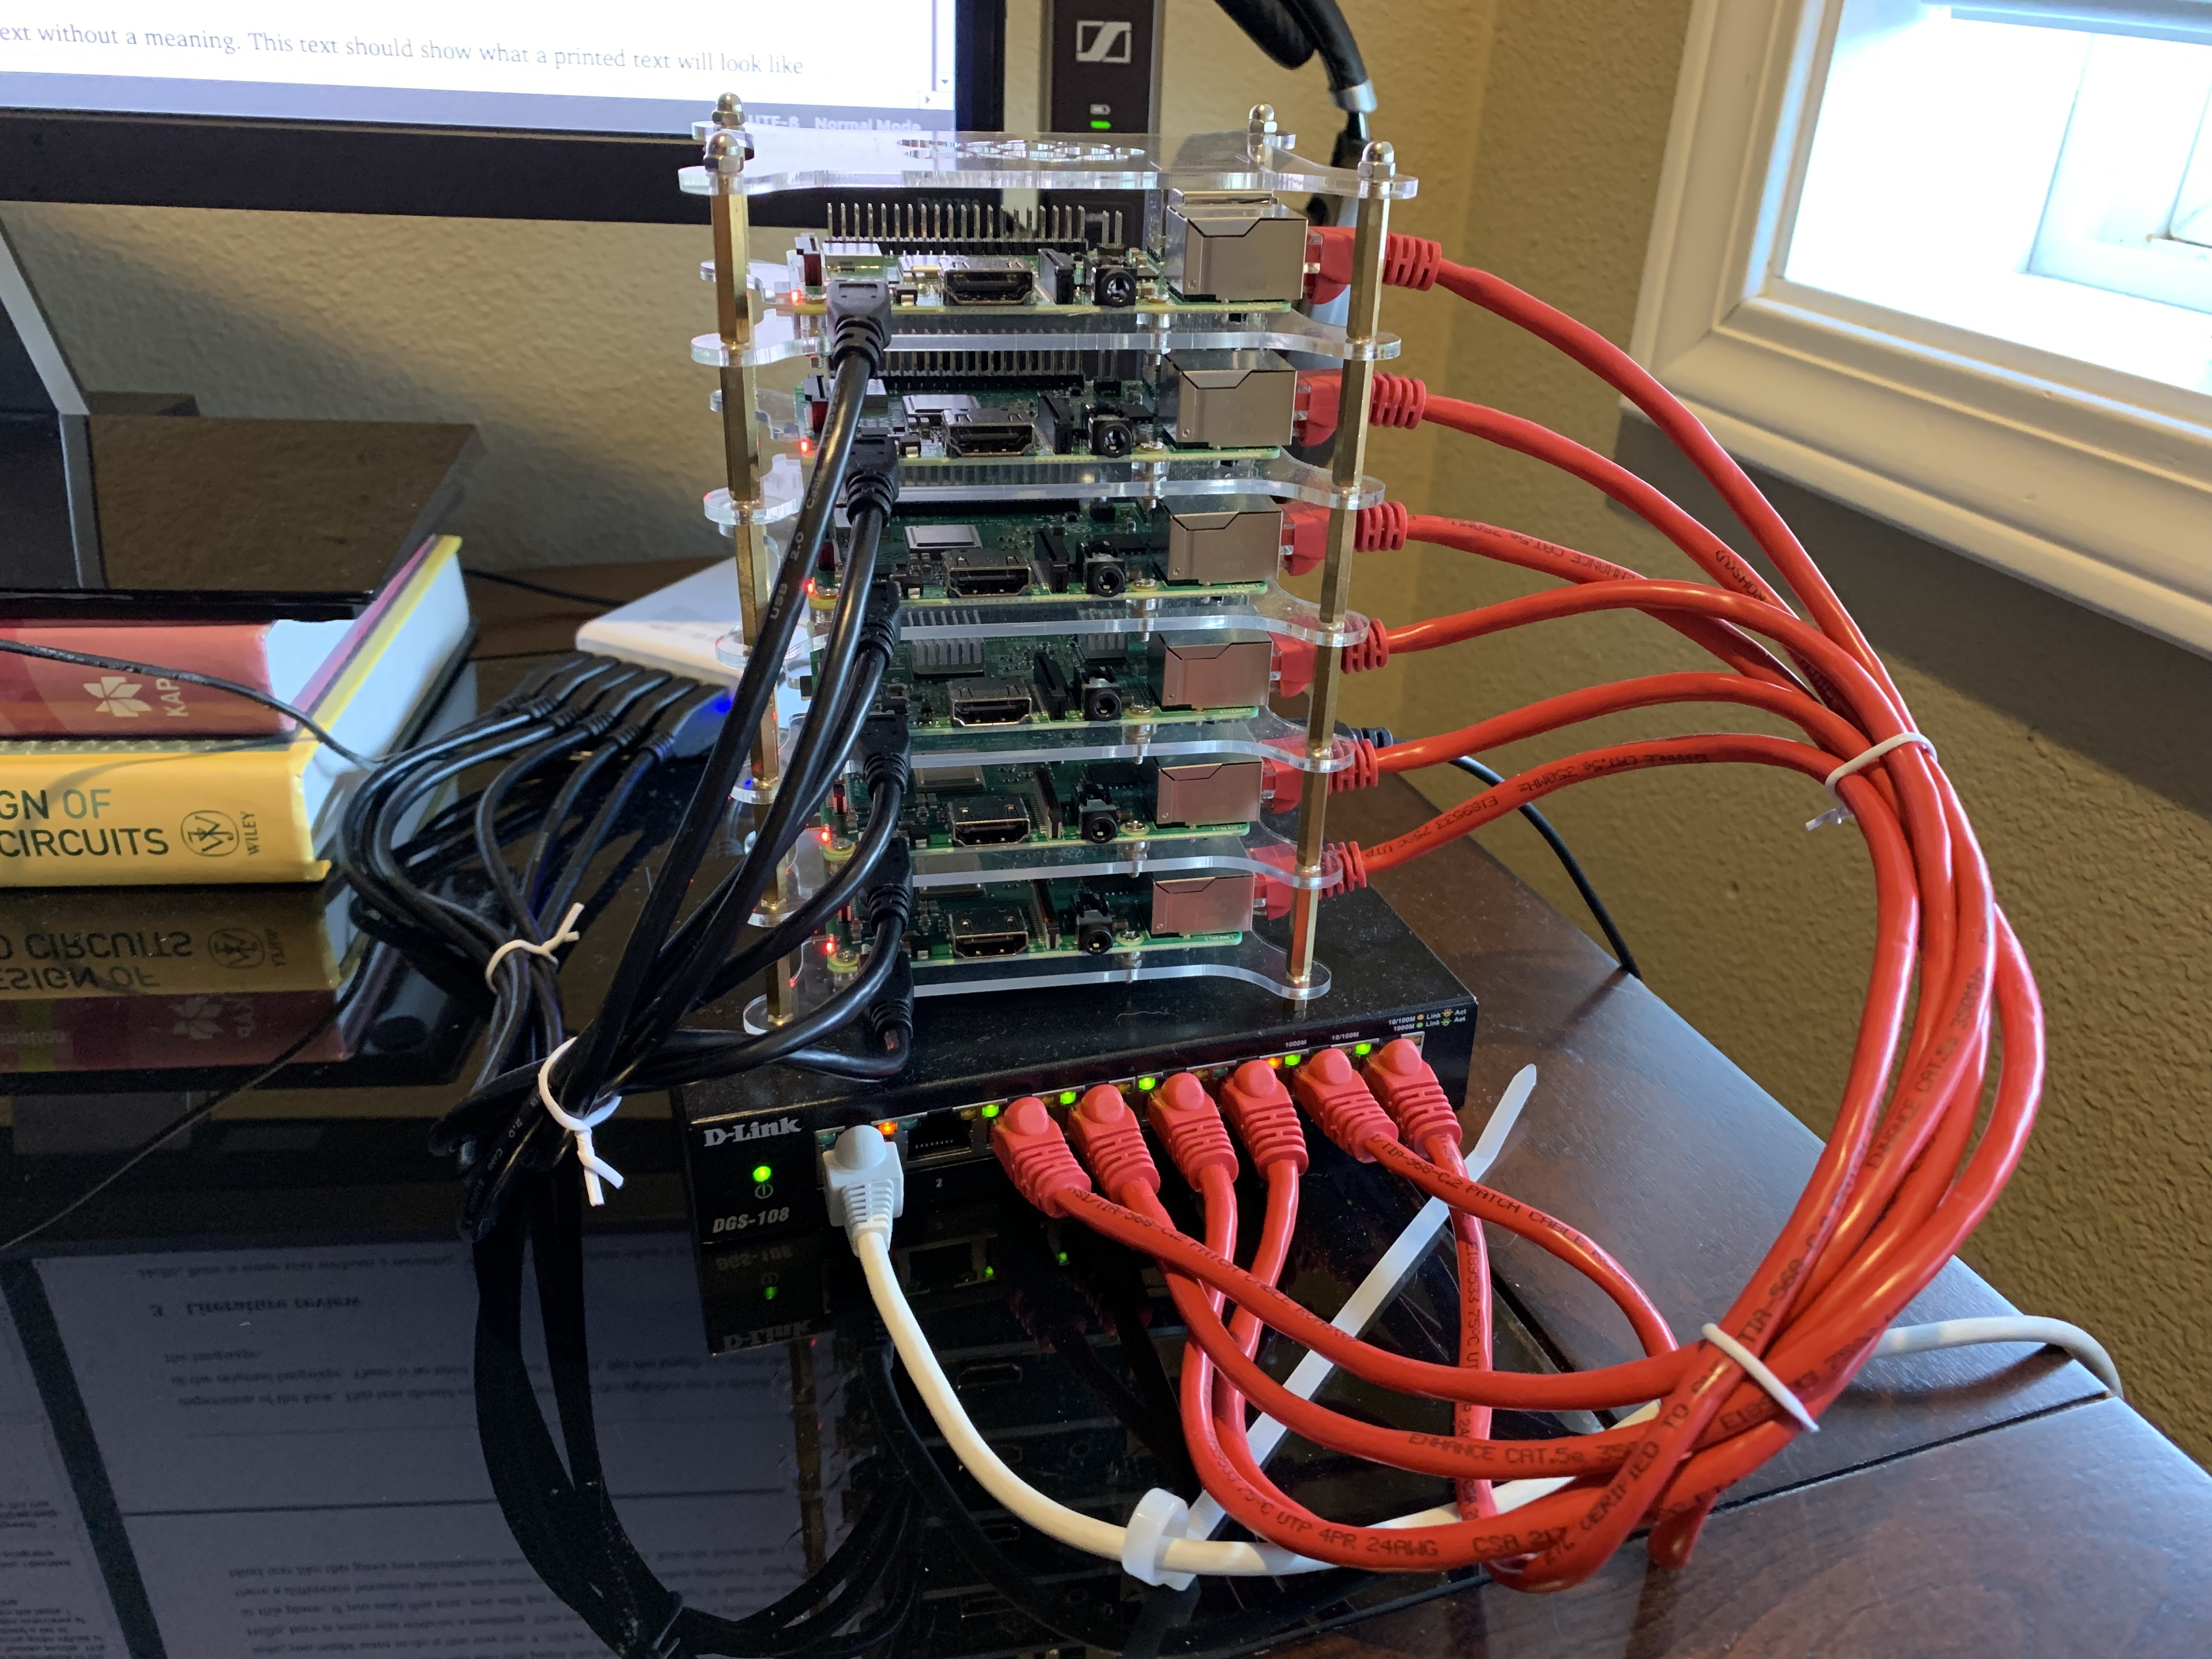
\includegraphics[width=\linewidth]{picluster.jpg}
  \caption{Raspberry Pi Cluster.}
  \label{fig:Raspberry Pi Cluster}
\end{figure}

For communication between nodes in the cluster, each Raspberry Pi was network through a D-Link DGS-108 8-port 10M/100M/1G Unmanaged Ethernet switch.

\subsection{Software}
I used the standard Raspian operating system which is built on the Debian Linux kernel. The Raspian version was GNU/Linux 9 Stretch and can be found here: \href{https://www.raspberrypi.org/downloads/raspbian/}{Raspian Downloads}. \\
\linespread{1}
The software I used included: \\
\begin{enumerate}
\item Open MPI 4.0.0
\item clang 7.0.1 \(tags/RELEASE_701/final\)
\item GNU back, version 4.4.21(1)-release (arm-unknown-linux-gnueabihf)
\end{enumerate}

\linespread{1.5}

%---------------------------------------------------------------------------------
% Theory
%---------------------------------------------------------------------------------
\section{Solution Algorithm - Backtracking}
There are many different algorithms available to find the solution to a general Sudoku puzzle.  These range from brute force(Backtrack) to extremely elegant(Don Knuth's Algorithm X.) Because my interest was in exploring in performance impact of programming techniques, using an algorithm which has inherently poor performance would help highlight differences in the programs.  Therefore, I chose to use the Backtracking algorithm.\\
The Back tracking is a recursive algorithm which follows these steps:
\linespread{1}
\textbf{btSolve(puzzle): }
\begin{enumerate}
\item Select any empty cell in the puzzle. If no empty cells, return PASS
\item If no numbers are left to try, return FAIL.
\item Select a number to try.
\item Validate the solution
\item If the solution is valid:
	\begin{enumerate}
	\item Call btSolve(puzzle)
	\item If return from btSolve is PASS, then return PASS.
	\item If return from btSolve is FAIL, go back to step 2.
	\end{enumerate} 
\item Go to step 2.
\end{enumerate}
\linespread{1.5}
As will be discussed in the analysis section, this algorithm does not lend itself easily to optimization through parallel methods - i.e. multi threading or multi processing.

\section{Program Descriptions and Data}
As stated, I used three different programming techniques to solve the Sudoku puzzles. An overview of each is included below.  Source code for each can be found at on GitHub at:\\ \href{https://github.com/jasongraalum/SudoSolv/}{https://github.com/jasongraalum/SudoSolv}. \\
\subsection{Serial}
The serial solution is identical to the standard algorithm included above. It ran on a single core and solved for the first possible solution. Even if the puzzle had multiple solutions, only the first was found and returned. The source code of the solver is shown in the Appendix A. \\

\begin{figure}
  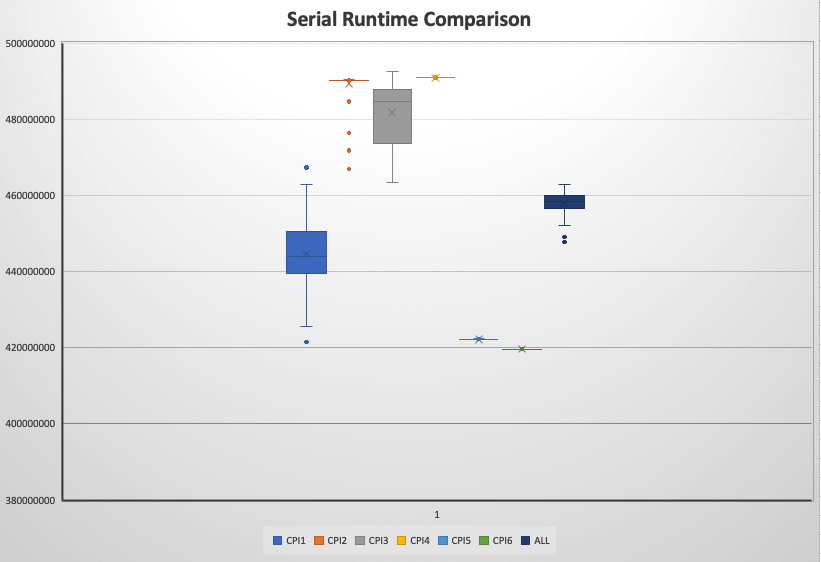
\includegraphics[width=\linewidth]{SerialRuntimeComparison.png}
  \caption{Serial Run-time Comparison}
  \label{fig:Serial Run-time Comparison}
\end{figure}
\subsection{Multi-threaded}
As was quickly discovered, the Backtrack algorithm does not lend itself easily to parallel optimization.  The one area that is straight forward is in the validation routine. To check if a given solution(partial or complete) is valid, three unique sections need to be checked for duplicate numbers: Rows, Columns and Blocks. In the threaded version of the code, I simply created a thread for each of theses for a total of three threads. The expected advantage is not large as the time spent in the verification routine is only a slightly greater than 50\% of the total program time. \\
At figure \ref{fig:SerialvPthread} shows, the Pthreaded version of the program is much slower(almost 3x slower) that the serial version.  This is due to the simple use of threading to run the verification setup as 3 parallel jobs. This speed up does not cover the overhead of the thread creation.  As pointed out during my presentation, creating a thread pool prior to calling the threads may provide some speed up.

\begin{figure}
  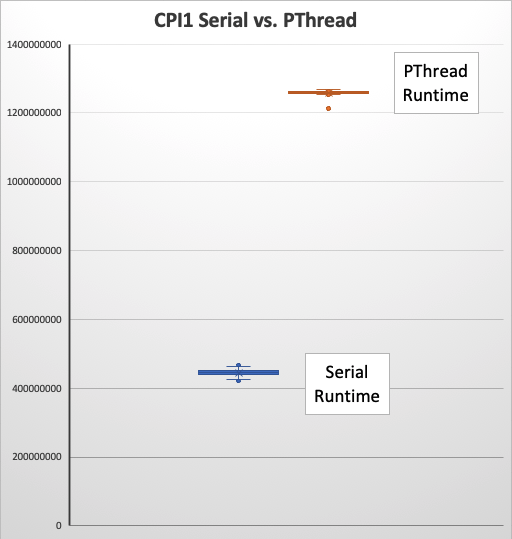
\includegraphics[width=\linewidth]{SerialvsPThread.png}
  \caption{Serial vs Pthread Run-time Comparison}
  \label{fig:SerialvPthread}
\end{figure}


\subsection{Multi-processor}
The mulit-processor solution is where I spent the majority of my effort.  I learned quite a bit about MPI programming and the difficulty of managing the interactions between the various processes. Overall, MPI showed the most promise with a runtime nearly equivalent to the serial version. I had begun working on a progam to generate all solutions to a given Sudoku puzzle as this would(I thought and still think) would lend its self much better to a parallel approach.  The trouble I ran into was synchronizing the various processes so that they didn't duplicate work or overwrite previous results.I would have liked to spend more time and effort analyzing and expanding the code, but alas, I ran out of time.

\begin{figure}
  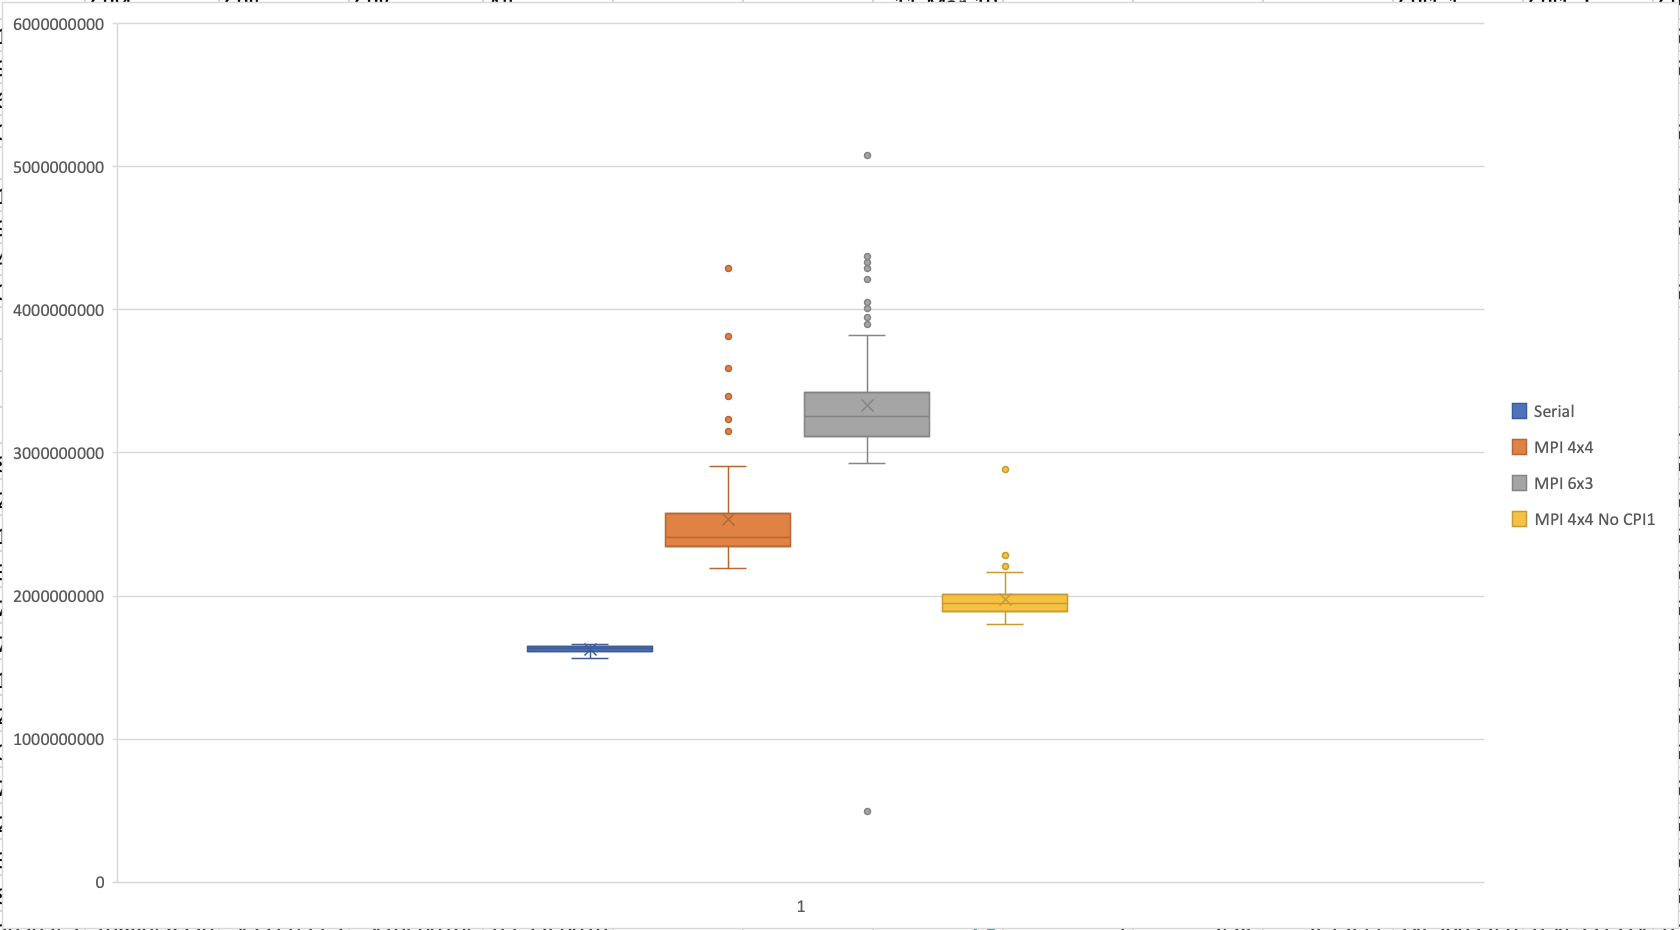
\includegraphics[width=\linewidth]{MPIRuntimeComparisons.png}
  \caption{MPI Runtime Comparison}
  \label{fig:MPIComparison}
\end{figure}

\section{Conclusions}
I had a great time with all the programming I did, which can be found on my GitHub page. However, the amount of programming got in the way of the analysis, so I feel the conclusions I can draw are a bit weak due to lack of analysis.  

%----------------------------------------------------------------------------------------
% Bibliography
%----------------------------------------------------------------------------------------
\newpage % Includes a new page

\pagenumbering{roman} % Changes page numbering to roman page numbers
%\bibliography{literature}

\bibliography{literature.bib} % Add the filename of your bibliography
\bibliographystyle{apsr} % Defines your bibliography style

% For citing, please see this sheet: http://merkel.texture.rocks/Latex/natbib.php

%----------------------------------------------------------------------------------------
% Appendix
%----------------------------------------------------------------------------------------
\newpage % Includes a new page
\section*{Appendix A: Serial Backtrack Algorithm Code}
\linespread{1}
\begin{verbatim}
#include "sudoSolvers.h"
#include "sudoSolvUtils.h"

int btSolve(Puzzle * p)
{
    return(addGuess(p, 0, 0));
}

int addGuess(Puzzle * p, int x, int y)
{
    // If cell already has a value
    if(getCell(p, x, y) != 0) {
        int new_x, new_y;
        new_x = (x + 1) % p->degree;
        new_y = new_x == 0 ? (y + 1) : y;

        // If x and y are the last cell, we have a solution
        if(new_y == p->degree) return(verifyPuzzle(p));

        // Call addGuess. If it returns greater than 0, we have a solution
        // If it returns less than 0, this guess_val isn't valid
        return(addGuess(p, new_x, new_y) > 0); 
    }

    Cell guess_val = 1;
    do {
        // Try a number
        setCell(p, x, y, guess_val);

        // If valid, increment cell indexes and call addGuess
        if(verifyPuzzle(p) > 0) {
            int new_x, new_y;
            new_x = (x + 1) % p->degree;
            new_y = new_x == 0 ? (y + 1) : y;

            // If x and y are the last cell, we have a solution
            if(new_y == p->degree) return(1);

            // Call addGuess. If it returns greater than 0, we have a solution
            // If it returns less than 0, this guess_val isn't valid
            if(addGuess(p, new_x, new_y) > 0) 
                return(1);
        }
        guess_val++;
        if(guess_val > p->degree) { 
            setCell(p, x, y, 0);
            return(-1);
        }
    } while(1);
}
\end{verbatim}
\linespread{1.5}
\section*{Appendix B: Multi-threaded Verification Function}
\linespread{1}
\begin{verbatim}
int verifyPuzzle()
{
    void *row_result, *col_result, *block_result;

    pthread_t *tid_row, *tid_col, *tid_block;
    tid_row = (pthread_t *)malloc(sizeof(pthread_t));
    tid_col = (pthread_t *)malloc(sizeof(pthread_t));
    tid_block = (pthread_t *)malloc(sizeof(pthread_t));

    // Check rows
    // For all rows
    // For all columns 0 to PDEGREE-1
    // For all columns  
    pthread_create(tid_row, NULL, checkPuzzleRows, NULL);

    // Check columns
    // For all columns
    // For all rows 0 to degree-1
    // For all rows  
    pthread_create(tid_col, NULL, checkPuzzleCols, NULL);

    // Check subblocks
    // Need to optimize this.
    // Loop for each subblock - there are PDEGREE subblocks
    pthread_create(tid_block, NULL, checkPuzzleBlocks, NULL);

    pthread_join(*tid_row, &row_result);
    pthread_join(*tid_col, &col_result);
    pthread_join(*tid_block, &block_result);

    int result = ((*(int *)row_result) + (*(int*)col_result) + (*(int *)block_result));

    return(result-6);
}
\end{verbatim}
\linespread{1.5}
\section*{Appendix C: Multi-processor Solution Function}
Some inconsequential code has been elided for brevity.\\
\linespread{1}
\begin{verbatim}
int main(int argc, char **argv)
{
    .
    .
    int numProcs, procId;
    MPI_Init(&argc, &argv);
    MPI_Comm_size(MPI_COMM_WORLD, &numProcs);
    MPI_Comm_rank(MPI_COMM_WORLD, &procId);

    Puzzle *p;

    char *inFilename;
    int repeats=1;

    // mpiPuzzle Datatype
    int puzzleBlocksCount = 4;
    int puzzleBlocksLength[4] = {1,1,1,1};
    MPI_Datatype puzzleTypes[4] = {MPI_UNSIGNED, MPI_UNSIGNED, MPI_UNSIGNED, MPI_UNSIGNED};
    MPI_Aint puzzleOffsets[4];
    MPI_Datatype mpiPuzzle;
    puzzleOffsets[0] = offsetof(Puzzle, degree);
    puzzleOffsets[1] = offsetof(Puzzle, setCount);
    puzzleOffsets[2] = offsetof(Puzzle, getCount);
    puzzleOffsets[3] = offsetof(Puzzle, cell);
    MPI_Type_create_struct(puzzleBlocksCount, puzzleBlocksLength, puzzleOffsets, puzzleTypes ,&mpiPuzzle);
    MPI_Type_commit(&mpiPuzzle);

    // mpiCell Datatype
    MPI_Datatype mpiCell;
    MPI_Type_create_resized(MPI_UNSIGNED, 0, sizeof(Cell), &mpiCell);
    MPI_Type_commit(&mpiCell);

    if(procId == 0) {
        if(argc != 3)
        {
            printf("Usage: sudoSolv <n repeats> <starting puzzle>\n");
            exit(-1);
        }

        repeats = atoi(argv[1]);
        inFilename = argv[2];

        printf("Repeats: %d\n", repeats);
        printf("Input file: %s\n", inFilename);

        time_data = (double *)malloc(sizeof(double)*repeats);
    }
    .
    .
    if(procId != 0)  
    {
        p = (Puzzle *)malloc(sizeof(Puzzle));
        p->degree = 0;
        p->cell = NULL;
        p->setCount = 0;
        p->getCount = 0;
    }

    for(int repeat = 0; repeat < repeats; repeat++) {
        if(procId == 0) {
            // Setup and print starting puzzle
            p = loadPuzzle(inFilename);
            if (p == NULL) {
                printf("Error loading puzzle. Exitting.\n");
            }
            //printPuzzle(p);
        }

        clock_gettime(CLOCK_REALTIME, &ts_realtime_start);
        //
        // Tranfer Puzzle to all other processes
        //
        MPI_Bcast(p, 1, mpiPuzzle, 0, MPI_COMM_WORLD);
        MPI_Barrier(MPI_COMM_WORLD);

        // Transmit puzzle cell contents
        int cell_count = p->degree*p->degree;
        if(procId != 0) p->cell = (Cell *)malloc(sizeof(Cell)*cell_count);
        MPI_Bcast(p->cell,cell_count, mpiCell, 0, MPI_COMM_WORLD);
        MPI_Barrier(MPI_COMM_WORLD);

        results[repeat] = btMPISolve(p, 0, 0, numProcs, procId);
        .
        .
        int totalSetCount;
        MPI_Reduce((void *)&p->setCount,(void*)&totalSetCount, 1, 
                              MPI_INT, MPI_SUM, 0, MPI_COMM_WORLD);
        int totalGetCount;
        MPI_Reduce((void*)&p->getCount,(void*)&totalGetCount, 1, 
                              MPI_INT, MPI_SUM, 0, MPI_COMM_WORLD);
	  .
	  .
    }

    if(procId == 0) {
        clock_gettime(CLOCK_REALTIME, &ts_totaltime_end);
        for(int repeat = 0; repeat < repeats; repeat++) {
            printf("%d,\t%d,\t%d,\t%d,\t%lf\n", repeat, results[repeat], sets[repeat], gets
                    [repeat], time_data[repeat]);
        }

        printf("Total time: %lf\n", (double)(1e9*(ts_totaltime_end.tv_sec-ts_totaltime_start.tv_sec)+(ts_totaltime_end.tv_nsec-ts_totaltime_start.tv_nsec)));
        //printPuzzle(p);
    }
    free(p->cell);
    free(p);
    MPI_Finalize();
    return 0;
}


#include "sudoMPISolvers.h"
#include "sudoMPISolvUtils.h"

int btMPISolve(Puzzle * p, int row, int col, int numProcs, int procId)
{
    int new_x, new_y;
    int * proc_res = (int*)malloc(sizeof(int));
    int *all_results = (int*)malloc(sizeof(int)*numProcs);

    // Get next empty cell, if no empty cell, return pass
    while(row < p->degree && col < p->degree && getCell(p, row, col) != 0) {
        row = (row + 1) % p->degree;
        col = (row == 0) ? (col + 1) : col;
    }
    if (col == p->degree) return(1);
    // setCell and Verify
    setCell(p, row, col, procId+1);
    *proc_res = verifyPuzzle(p);
    setCell(p, row, col, 0);

    // Gather all results
    MPI_Allgather(proc_res,1,MPI_INT,all_results,1,MPI_INT, MPI_COMM_WORLD);
    MPI_Barrier(MPI_COMM_WORLD);

    // Pick first passing result
    for(int i = 0; i < numProcs; i++)
    {
        // setCell
        if(all_results[i] > 0) {
            setCell(p, row, col, i+1);
            int next_proc_res = btMPISolve(p, row, col, numProcs, procId);

            // If solver return is pass, return pass
            if(next_proc_res > 0) return(1);
            setCell(p, row, col, 0);
        }
        // If solver return is fail, try next passing result
    }
    return(0);
}


\end{verbatim}

%---------------------------------------------------------------------------------

\end{document}
